\chapter{L'implementazione}

\section{Le applicazioni cross-platform}
Negli ultimi anni, i dispositivi mobili sono diventati sempre più parte integrante della nostra vita, grazie al progresso tecnologico e all'abbattimento dei prezzi, oggi costituiscono un bene alla portata di tutti. \\
La possibilità di scegliere tra una vasta gamma di smartphone diversi per caratteristiche e produttore, ha reso più complicata la vita delle aziende informatiche che sono costrette a considerare l'eterogeneità dei vari sistemi operativi in circolazione.\\
\begin{figure}[H]
	\centering
	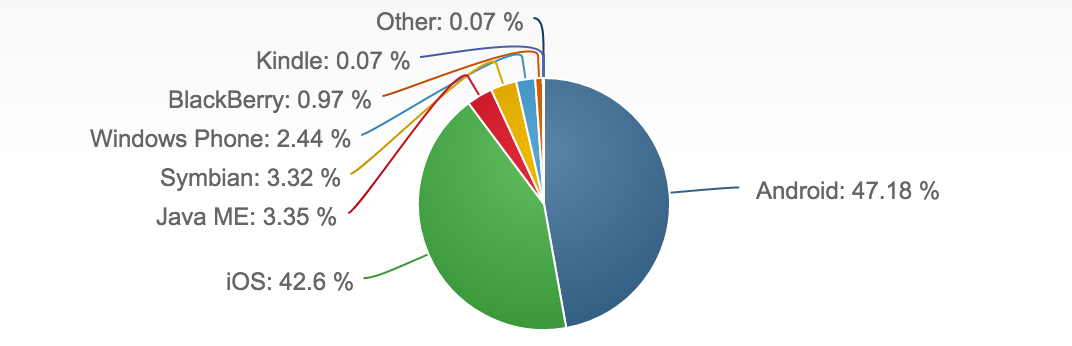
\includegraphics[scale=0.7]{Implementazione/os.png}
	\caption{Utilizzo dei vari OS su scala mondiale}
	\label{fig:os_mobile}
\end{figure}
\newpage
Chi sviluppa applicazioni mobili, può scegliere tra due approcci:
\begin{enumerate}
\item \textbf{Scegliere uno degli OS mobile} e implementare l'applicazione utilizzando il linguaggio nativo.
\item \textbf{Scegliere un framework }che, utilizzando un meta-linguaggio, sia in grado di generare diverse versioni dell'applicazione per i relativi OS.
\end{enumerate}
I diversi approcci forniscono rispettivamente pro e contro. Per il primo i vantaggi sono una maggiore velocità del sistema, la possibilità di creare un'interfaccia rispettando il look and feel nativo e pochi problemi di compatibilità. Lo svantaggio è invece legato alla \textbf{bassa portabilità}, l'applicazione andrà riscritta completamente per dispositivi con diversi OS. \\
Il principale vantaggio del secondo approccio, è invece la possibilità di riutilizzare lo stesso codice per generare varie versioni dell'applicazione per diversi OS, questo a discapito di una minore velocità del sistema se l'applicazione fosse sviluppata nel linguaggio nativo. \\
Considerando il contesto d'uso del sistema ( vedi \ref{contesto}), è chiaro che la nostra applicazione dovrebbe poter essere installata su qualsiasi dispositivo (ndr l'idea di salvare vite con un certo OS non è delle più nobili), di conseguenza si è adottato tale approccio.\\
La filosofia \textit{"Write once, run anywhere"}, non è un concetto nuovo nell'informatica, lo slogan fu ideato dalla Sun Microsystems per descrivere un linguaggio (Java) in grado di essere eseguito su diverse macchine. Nel corso degli anni diverse software-house hanno realizzato dei framework in grado di fare questa "magia", sostanzialmente ne estitono due tipi:
\begin{itemize}
\item \textbf{ I Cross-Compiling:} si scrive l'applicazione in un certo linguaggio, successivamente un framework riesce a compilarlo per le diverse piattaforme (Appcelerator Titanium1, Corona SDK2, Xamarin Monotouch3); Solitamente sono framework professionali e a pagamento.
\item \textbf{I Browser-Embedding:} più recenti, consentono di sviluppare il codice con le tecnologie del web (HTML5, CSS3, Javascript), l'applicazione verrà avviata nel dispositivo mobile all'interno di un browser (PhoneGap, Apache Cordova).
\end{itemize} 
Ancora una volta è stato scelto il secondo approccio, nello specifico il framework PhoneGap.

\section{PhoneGap}
\label{phonegap}
Phonegap è un framework di sviluppo mobile prodotto da Nitobi e acquistato successivamente da Adobe Systems. Permette ai programmatori software di creare applicazioni per dispositivi mobili utilizzando esclusivamente HMTL, CSS e Javascript invece di utilizzare linguaggi nativi come Object-C e C++. Il risultato sono applicazioni ibride, nel senso che non sono né del tutto native (perché tutto il rendering del layout è fatto tramite viste web e non tramite i framework UI delle piattaforme native) né del tutto web-application (perché non sono applicazioni solo web, ma hanno anche accesso alle funzioni interne dei device tramite le API). \\
Il software alla base di PhoneGap è \textit{Apache Cordova} ed è open source. \\
\begin{figure}[H]
	\centering
	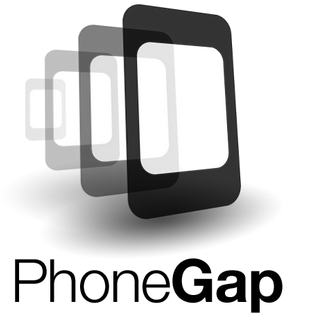
\includegraphics[scale=0.6]{Implementazione/logo_phonegap.png}
	\caption{Logo del framework PhoneGap}
	\label{fig:logo_phonegap}
\end{figure}
Presentato la prima volta in un evento iPhoneDevCamp a San Francisco, PhoneGap ha vinto il premio People's Choice Award alla conferenza O'Reilly Media Web nel 2009. Il framewotk PhoneGap viene utilizzato da molte piattaforme  di sviluppo software come ViziApps, Worklight, Convertico e appMobi. \\
Il 4 ottobre 2011 Adobe annuncia ufficialmente l'acquisizione della Nitobi Software. In concomitanza il codice PhoneGap ha contribuito con la Apache Software Foundation ad iniziare un nuovo preocetto chiamato Apache Cordova.
\newpage
PhoneGap non è altro che un modulo software che permette agli sviluppatori di incorporare le loro applicazioni web all'interno di applicazioni native di diverse piattaforme. Le applicazioni che utilizzano questo framework sono scritte in HTML5, CSS3 e Javascript e il collegamento con le livrerie native, specifiche di ogni piattaforma, è fatto tramite le API che mette a disposizione il framework.
PhoneGap fa quindi da ponte tra il sistema operativo e la web application realizzata dallo sviluppatore. Indipndentemente dalla piattaforma sottostante esisterà un modo per invocare le API native mediante funzioni Javascript. \\
Il programmatore quindi utilizzerà le API fornite da PhoneGap per accedere alle risorse hardware e software del device in modo da aggiungere le funzionalità di base al motore JAvascript e renderle facilmente utilizzabili come se fossere vere e propri metodi di una libreria. Dopo la compilazione, che avviene tramite il servizio cloud \textbf{PhoneGap Build} (Figura \ref{fig:phonegap_build}), viene generato un pacchetto internamente composto da due elementi principali con differenti responsabilità che però cooperano tra loro per fornire delle funzioni a valore aggiunto. In pratica esiste un runtime basato su WebKit4 in cui vengono iniettate le componenti statiche; il risultato sarà un pacchetto composta da due elementi principali con differenti responsabilità che però cooperano tra loro per fornire delle funzioni a valore aggiunto. Nel caso specifico il runtime si occupa di dialogare direttamente con il dispositivo e le parti statiche offrono l'interfaccia verso l'utente. L'uso di Javascript e Ajax consente poi di rendere le applciazioni più complesse e dinamiche.
\begin{figure}[H]
	\centering
	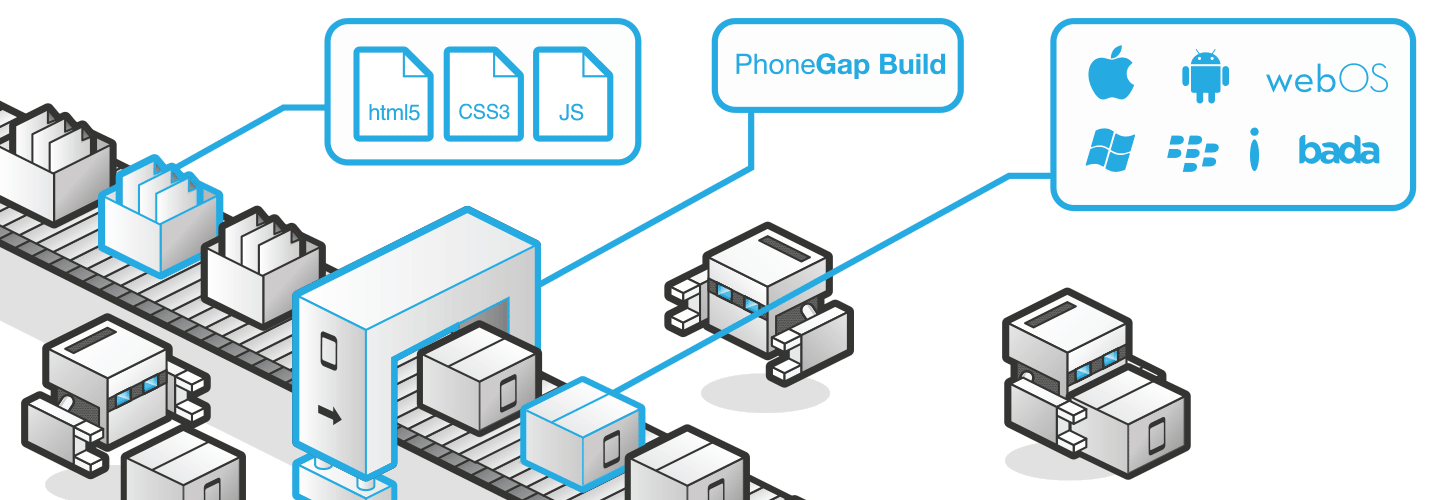
\includegraphics[scale=0.3]{Implementazione/phonegap_build.png}
	\caption{Logo del framework PhoneGap}
	\label{fig:phonegap_build}
\end{figure}

\newpage
Ora illustriamo mediante la Figura \ref{fig:architettura_phonegap} come è strutturata l'architettura PhoneGap. Partendo dal basso verso l'alto, si può notare che la parte in blu è quella del sistema operativo della piattaforma nativa che si trova sui vari device. Al livello immediatamente successivo troviamo il framework PhoneGap (in grigio) che ci viene fornito insieme alle API Javascript. Da notare il rettangolo arancione che rappresenta l'embedded browser che incapsula la web application e le API. Di default il browser viene aperto esternamente all'applicazione. Di conseguenza ad ogni richiesta di una pagina web avviene l'apertura di un bottone fornito dal browser. In pratica si rende impossibile notare che si tratta di un browser e quindi di una pagina web. Ciò rende l'applicazione più simile ad un applicazione nativa.\\
Infine, in verde è evidenziata la parte a carico dello sviluppatore che è la vera e propria web application, realizzata all'interno del framework PhoneGap.
\begin{figure}[H]
	\centering
	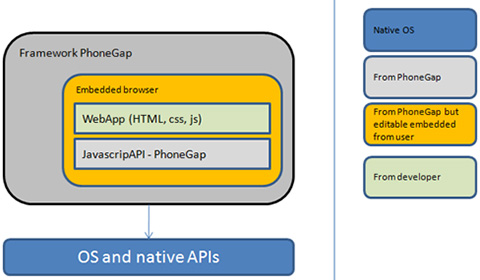
\includegraphics[scale=0.9]{Implementazione/phonegap_architettura.jpg}
	\caption{Architettura di un'applicazione realizzata con PhoneGap}
	\label{fig:architettura_phonegap}
\end{figure}

Come detto PhoneGap mette a disposizione del programmatore, una serie di API per l'accesso all'hardware nativo del device. Bisogna tenere conto però che non tutte le piattaforme hanno a disposizione gli stessi sensori e che occorre prestare molta attenzione nel caso in cui il building dell'applicazione è fatto su piattaforme diverse. Il framework, infatti, offre supporto per ogni piattaforma degna di essere presa in considerazione ovvero: Android, iOS, Symbian, WebOS, Blackberry etc. Non tutte le piattaforme son però supportate allo stesso modo. La seguente tabella (Fig \ref{fig:tabella_api} )
riassume lo stato dell'arte riguardo la compatibilità e l'accessibilità che il framework offre verso i sensori presenti nei diversi device, equipaggiati da diversi OS.

\begin{figure}[H]
	\centering
	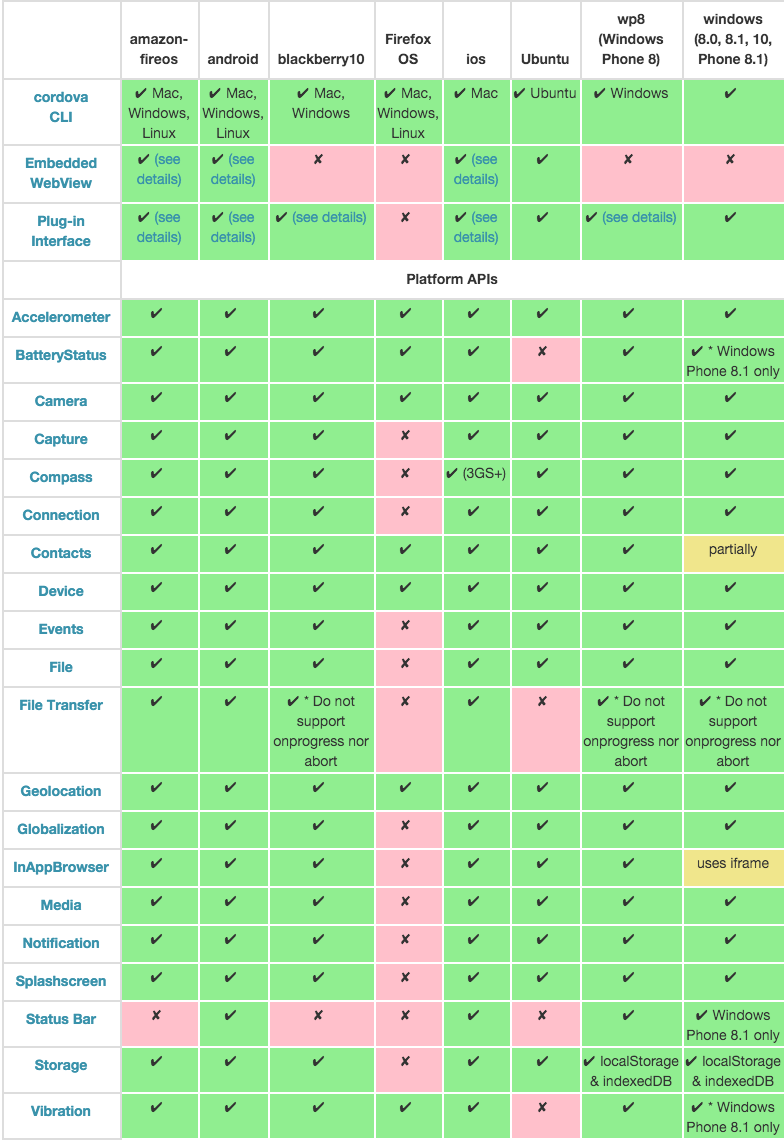
\includegraphics[scale=0.8]{Implementazione/phonegap_api.png}
	\caption{Le API e il loro supporto per le varie piattaforme}
	\label{fig:tabella_api}
\end{figure}

\section{Ratchet}
Il solo utilizzo del framework PhoneGap non è sufficiente per realizzare un'applicazione degna di nota. L'interfaccia grafica costituisce un'elemento fondamentale nelle moderne applicazioni mobili. Inoltre, se ben progettata, contribuisce ad aumentare la user experience \cite{EXPERIENCE} e in generale l'usabilità del sistema stesso. A tale proposito è stato utilizzato il framework opens source \textbf{Ratchet}.

\begin{figure}[H]
	\centering
	
\includegraphics[scale=0.8]{Implementazione/ratchet_logo.png}
	\caption{Il logo del framework Ratchet}
	\label{fig:logo_ratchet}
\end{figure}

I componenti offerti da questo strumento sono responsive e appositamente progettati per i dispositivi mobile ed il loro utilizzo è tanto semplice quanto efficace; analogamente ad altri progetti di successo, come Bootstrap, i componenti possono essere inclusi nell'interfaccia semplicemente aggiungendo codice HTML e stili CSS. La combinazioe di questo tool con un altro in grado di accedere al DOM (Document Object Model) dell'applicazione (vedi \ref{phonegap}), nel nostro caso si è utilizzato\textit{ JQuery}, permette di realizzare applicazioni molto simili a quelle native.\\
